%%%%%%%%%%%%%%%%%%%%%%%%%%%%%%%%%%%%%%%%%%%%%%%%%%%%%%%%%%%%%%%%%%%%%%%%%%%%%
%%%
%%% File: thesis.tex, version 1.9, May 2016
%%%
%%% =============================================
%%% This file contains a template that can be used with the package
%%% cs.sty and LaTeX2e to produce a thesis that meets the requirements
%%% of the Computer Science Department from the Technical University of Cluj-Napoca
%%%%%%%%%%%%%%%%%%%%%%%%%%%%%%%%%%%%%%%%%%%%%%%%%%%%%%%%%%%%%%%%%%%%%%%%%%%%%

\documentclass[12pt,a4paper,twoside]{report}     
\usepackage{cs}              
\usepackage{times}
\usepackage{graphicx}
\usepackage{latexsym}
\usepackage{amsmath,amsbsy}
\usepackage{amssymb}
\usepackage[matrix,arrow]{xy}
\usepackage[T1]{fontenc}
\usepackage{ae,aecompl}
%\usepackage{shortcut} %definitii pentru diacritice; 
\usepackage{amstext}
\usepackage{graphics}
\usepackage[T1]{fontenc}
\usepackage{ae,aecompl}
\usepackage{algorithm}
%\usepackage{algorithmic}
\usepackage{color}
\usepackage{color}
\usepackage{bytefield}
\usepackage{listings} 

\usepackage[hyphens]{url}
\usepackage[hidelinks]{hyperref}
\hypersetup{breaklinks=true}
\urlstyle{same}
\usepackage{cite}



% \mastersthesis
\diplomathesis
% \leftchapter
\centerchapter
% \rightchapter
\singlespace
% \oneandhalfspace
% \doublespace

\renewcommand{\thesisauthor}{Áron KATONA}    %% Your name.
\newcommand{\thesisauthorgroup}{30433}    %% Your group.
\renewcommand{\thesismonth}{}     %% Your month of graduation.
\renewcommand{\thesisyear}{2020}      %% Your year of graduation.
\renewcommand{\thesistitle}{Automated irrigation station with integrated RESTful web server} 
\renewcommand{\thesissupervisor}{}
\newcommand{\department}{\bf FACULTY OF AUTOMATION AND COMPUTER SCIENCE\\
COMPUTER SCIENCE DEPARTMENT}
\newcommand{\thesis}{}
\newcommand{\utcnlogo}{
\includegraphics[width=15cm]{img/tucn.jpg}}

\newcommand{\uline}[1]{\rule[0pt]{#1}{0.4pt}}
%\renewcommand{\thesisdedication}{P\u{a}rin\c{t}ilor mei}

\begin{document}
%\frontmatter
%\pagestyle{headings}

\newenvironment{definition}[1][Defini\c{t}ie.]{\begin{trivlist}
\item[\hskip \labelsep {\bfseries #1}]}{\end{trivlist}}



%\thesistitle                    %% Generate the title page.
%\authordeclarationpage                %% Generate the declaration page.


\begin{center}
\utcnlogo

\department

\vspace{4cm}

{\bf \thesistitle} %LICENSE THESIS TITLE}

\vspace{1.5cm}


\vspace{6cm}

Name: {\bf \thesisauthor} 

Group: {\bf \thesisauthorgroup}

\vspace{1cm}

https://github.com/katonaaron/irrigation-station

\vspace{2cm}
{\bf \thesisyear}
\end{center}

\thispagestyle{empty}
\newpage

\pagenumbering{roman}
\setcounter{page}{1}



\tableofcontents
\newpage

\pagenumbering{arabic}
\setcounter{page}{1}
\pagestyle{headings}

 
\chapter{Introduction}



\chapter{Bibliographic research} 

As described in chapter \ref{sec:not_new}, there are already solution for the given problem, however each implementation must be tailored to the specific use cases.




\section{Controller}

For controlling the moister level by reading a sensor value and activating  a pump the following approaches were observed:

\subsection{Operational amplifier based} 

A reference voltage is set to the desired value. The other input of the amplifier is connected to the sensor output. The amplifier saturates the value to 0V or 5V based on the result of comparison between the two voltages. The output of the amplifier enables the water pump.

\subsection{Microcontroller based}

The comparison of the two voltages can be done by the program running on the microcontroller. It can also activate the enable signal for the pump. 

\subsection{Mixed}

The two methods can be mixed: the microcontroller can set the reference value, and the operational amplifier can compare it with the sensor value and trigger the pump.


\subsection{Comparison}

The operational amplifier approach is really cheap and robust. However it lacks the support for setting up the reference value remotely. 

The microcontroller is more expensive, and less reliable, because of the programming errors that might occur. Moreover because of the delay between two successful verifications the reaction time is greater than for the other approach. However the advantage is that the microcontroller can delay some processes e.g. sensor verification, time between successive pumps. This can be useful in a real application.

The mixed solution seems to be ideal from a functional point of view, because this way the reference value can be changed remotely by the user, and the controlling part is ``bug-free'' and responsive. This approach's cost is the sum of the costs of the previous two methods.

\section{Water source}

\subsection{Water tank}

One could store the water in a tank or a bucket. In this approach a water pump transmits the water from the tank to the plant. This method is ideal for indoor plants. However the user must take care of the refilling of the water tank.

\subsection{Pipes}

One could connect the irrigation system to the water pipe network of its home. This way the user does not have to bother anymore with verifying the water level of a water tank. For this, a solenoid valve can be used which can turn on or off the flow of water between two pipes. This method is ideal for outdoor plants.

\subsection{Comparison}

From the point of view of the price a solenoid valve is usually more expensive than a water pump. However a single one of it can control the irrigation of many outdoor plants. A water pump is much cheaper,  but for each plant a separate pump must be bought which increases the total cost.

From a functional point of view, the flow rate cannot be configured for a solenoid valve. It just enables or disables the flow of water between two pipes. This way, unless the designer knows how to decrease the pressure in the output pipe (maybe programatically), the valve cannot be used for indoor plants, because of the too much quantity of water. Therefore it would serve a better purpose for outdoor plants where an overshoot would not cause unpleasant moments to the user.

The speed of a water pump can be set programatically therefore it can be used for a more refined controller.



\section{Communication interface}

The type of the communication interface greatly defines the optimal components that should be used.

\subsection{Local configuration}

If the system should be configured by buttons, potentiometers and other circuit components which requires the user to be present physically, one should choose a microcontroller which:

\begin{enumerate}
 \item has enough analog pins and/or digital pins
 \item costs the less
\end{enumerate}



\subsection{Wi-Fi communication}

For wireless communication the approaches differ by the place the web server code is uploaded.

\subsubsection{Microcontroller + Wi-Fi module + AT commands}

One could use any microcontroller which supports serial communication for this approach. In this case a Wi-Fi module is required (e.g. ESP8266) which can communicate through the serial port. The AT firmware is designed for the ESP8266 chip, and it allows the microcontroller to perform a wast number of operations. The advantage of this approach is that the Wi-Fi module is ready for use, and doesn't have to be programmed. This disadvantage is that the commands are limited. For example to detect in the microcontroller which endpoint was called, one must parse the data received through the serial port byte-by-byte.

\subsubsection{Microcontroller + Wi-Fi module + Custom firmware}

This approach is similar to the previous one, with the difference that the designer uploads a custom firmware to the Wi-Fi module. This way the designer can exploit all the functionalities of the module. However it requires double amount of time to implement the communication between the two components.


\subsubsection{Microcontroller with integrated Wi-Fi module}

One could use a microcontroller which has an integrated Wi-Fi receiver and transmitter. Such microcontroller is the NodeMCU. This way the designer can use a higher level API for providing HTTP endpoints (compared to the first approach) and also the server speed is increased because of the lack of serial communication. Therefore all the network capabilities can be used, and the development time is also reduced (compared to the second approach) because all the logic can be programmed into a single chip.

A disadvantage might be that the NodeMCU has only a single analog input.

\subsubsection{Additional notes for Wi-Fi module based implementation}

The ESP8266 works on 3.3V voltage level. Therefore voltage level shifters are needed for its VIN, RX and TX pins in order to work with 5V level circuits, like the Arduino Mega. Moreover the Arduino cannot supply sufficient current to power it on , therefore the VIN must be connected to the external power source.

This can provide some unfortunate moments for the designer after the realization that more components must be bought and interconnected. However one can buy the so called Wi-Fi shields, which can be placed directly on the microcontroller without any additional configuration. The disadvantage of this method is that the shield may not provide access to some important pins of the microcontroller.




\subsection{Bluetooth communication}

Bluetooth communication can also be considered. The main disadvantages compared to the Wi-Fi solution is that it reduces the communication range, and the client must pair its device with the system.







\section{Moisture sensor calibration}

Considering a linear capacitive moisture sensor the following approaches can be taken.

\subsection{Measuring the extreme values}

Being the sensor linear, one could measure the moisture level when the soil of the plant is totally dry and when it's totally wet. Any sensor reading will be in this interval, thus the user can specify a desired percentage of the moisture level.

The disadvantage of this approach is that the voltage readings  highly depend on the volume and the composition of the soil. Therefore for each plant this calibration must be done individually.


\subsection{Predicting volumetric water content}

Another approach is to find the linear function which maps the voltage readings to the ration between the volume of the water and the volume of the soil. This way the calibration is down per types of soils and not per plants. Moreover the volume of the soil would not affect the results.

This approach is more time consuming, but the accuracy is greater. More details can be found in \cite{Hrisko20}.

\chapter{Proposed solution and Implementation} 

\section{Chosen solution}

The following decisions and use cases were considered:

\begin{itemize}
 \item The subjects of the irrigation are indoor plants.
 \item The water source is a bucket.
 \item The controller is implemented using an Arduino Mega microcontroller.
 \item The controller must be calibrated for each plant: one must measure the moisture in the soil in both extreme cases.
 \item The user can configure the controller parameters: e.g. the threshold moisture level.
 \item The configuration interface is a REST web server, hosted on a ESP8266 Wi-Fi shield with the AT firmware.
\end{itemize}

The following features were also included in the system:

\begin{itemize}
 \item Persisting the configuration parameters in EEPROM
 \item Allowing the user to set the extreme values by pressing buttons
 \item Displaying the moisture percentage or eventual errors on a seven segment display
\end{itemize}






\section{Algorithms}

\subsection{Controlling the moisture level}
\label{sec:control_fsm}

\begin{figure}[ht]
    \centering
    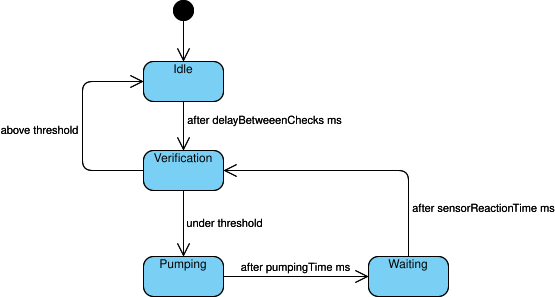
\includegraphics[width=\linewidth]{img/Irrigation station controller state diagram.png}
    \caption{The state diagram of the moisture level controller}
    \label{fig:controller_state_diagram}
\end{figure}

The controller can be considered as a state machine (figure \ref{fig:controller_state_diagram})  which changes states based on the sensor readings and on the timing parameters configured by the user.

In the \textbf{idle state} the controller waits. The \verb|delayBetweenChecks| parameter specifies the duration the controller stays in this state. After that it moves to the verification state.

In the \textbf{verification state} the sensor value is read, converted to percentage based on the saved extreme values, and  finally, it is compared with the threshold value. In case it is lower, the pumping state follows, in the other case the controller moves back to the idle state.

In the \textbf{pumping state} the pump is enabled and the water flows from the tank to the plant. The duration of pumping is given by the \verb|pumpingTime| parameter. After that it moves to the waiting state.

In the \textbf{waiting state} the controller waits for the sensor to react to the water flowing from the pump. The duration is given by the \verb|sensorReactionTime| parameter. Then it moves to the verification state.

\subsection{Parsing HTTP requests byte-by-byte}
\label{sec:http_fsm}

From the HTTP requests only the request type and the endpoint are considered, the rest is ignored. Therefore another state machine was used which reads the characters from the Wi-Fi module, and saves only these two strings into separate variables. The state transitions happen on reading the \verb|' '| character.





\section{Implementation}

\section{Hardware} 

\begin{figure}[ht]
    \centering
    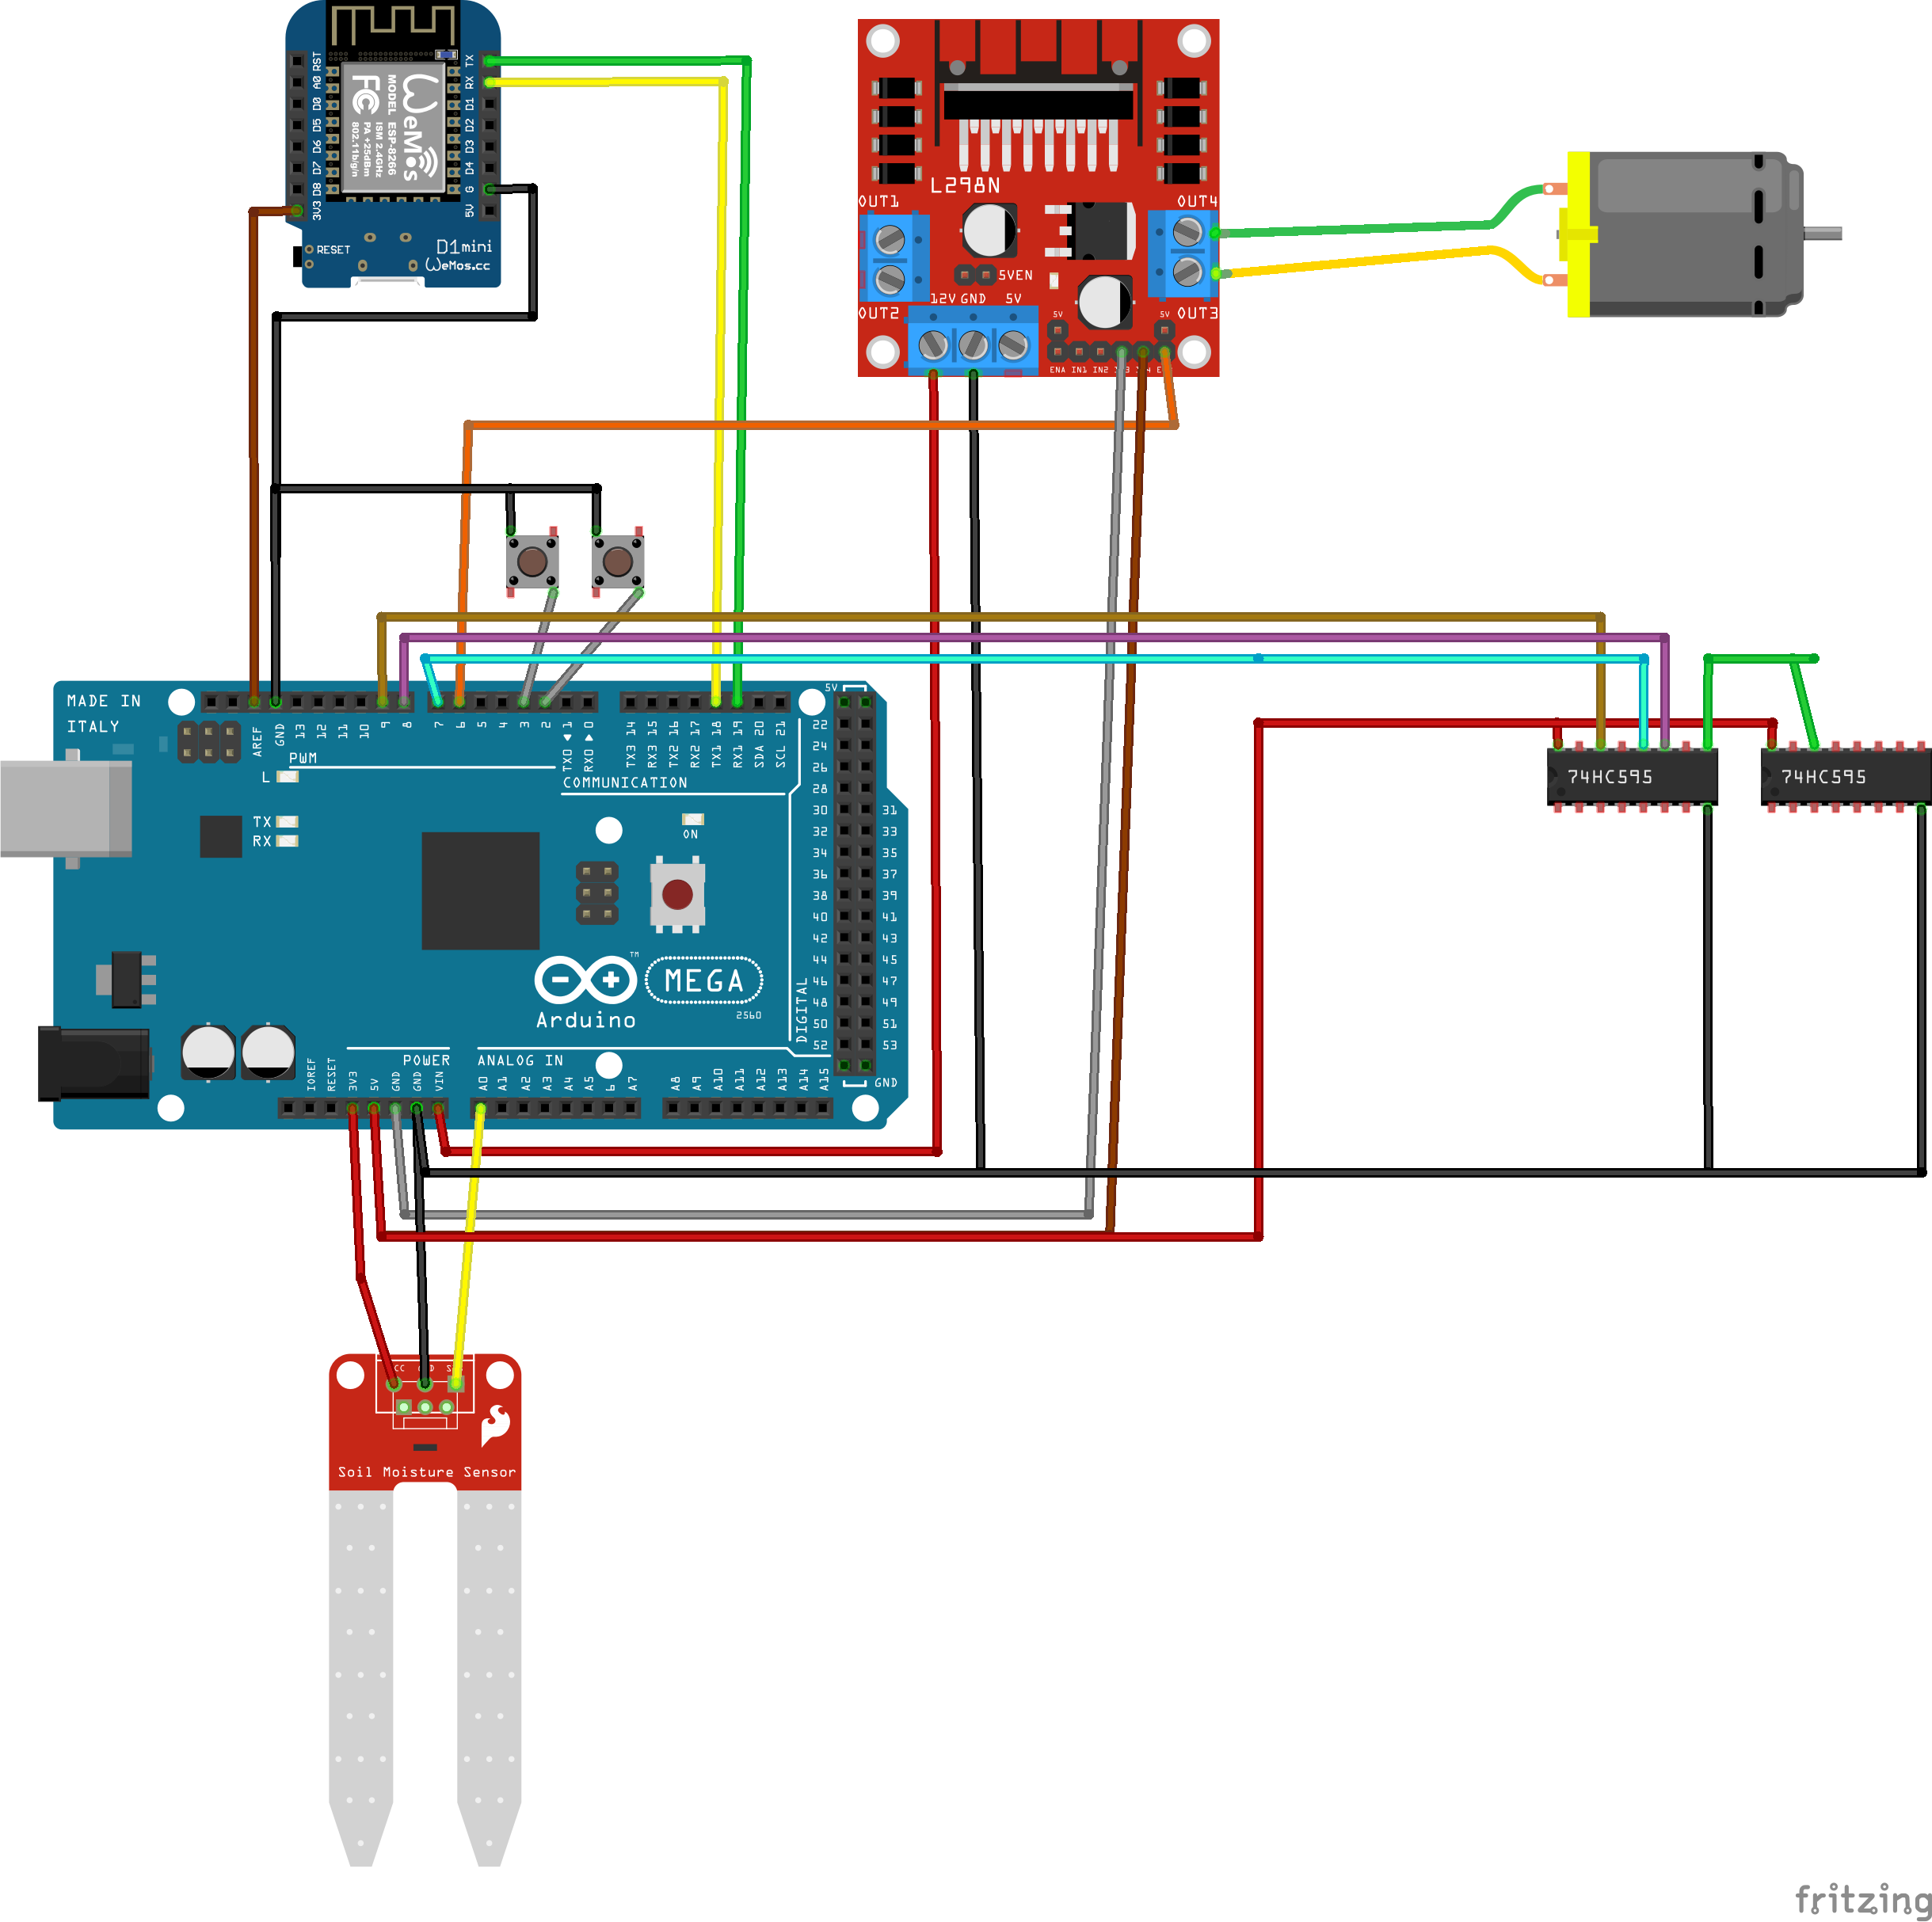
\includegraphics[width=\linewidth]{img/IrrigationStationHardware.png}
    \caption{The overview of the hardware components and their interconnections}
    \label{fig:hardware_diagram}
\end{figure}

\begin{figure}[ht]
    \centering
    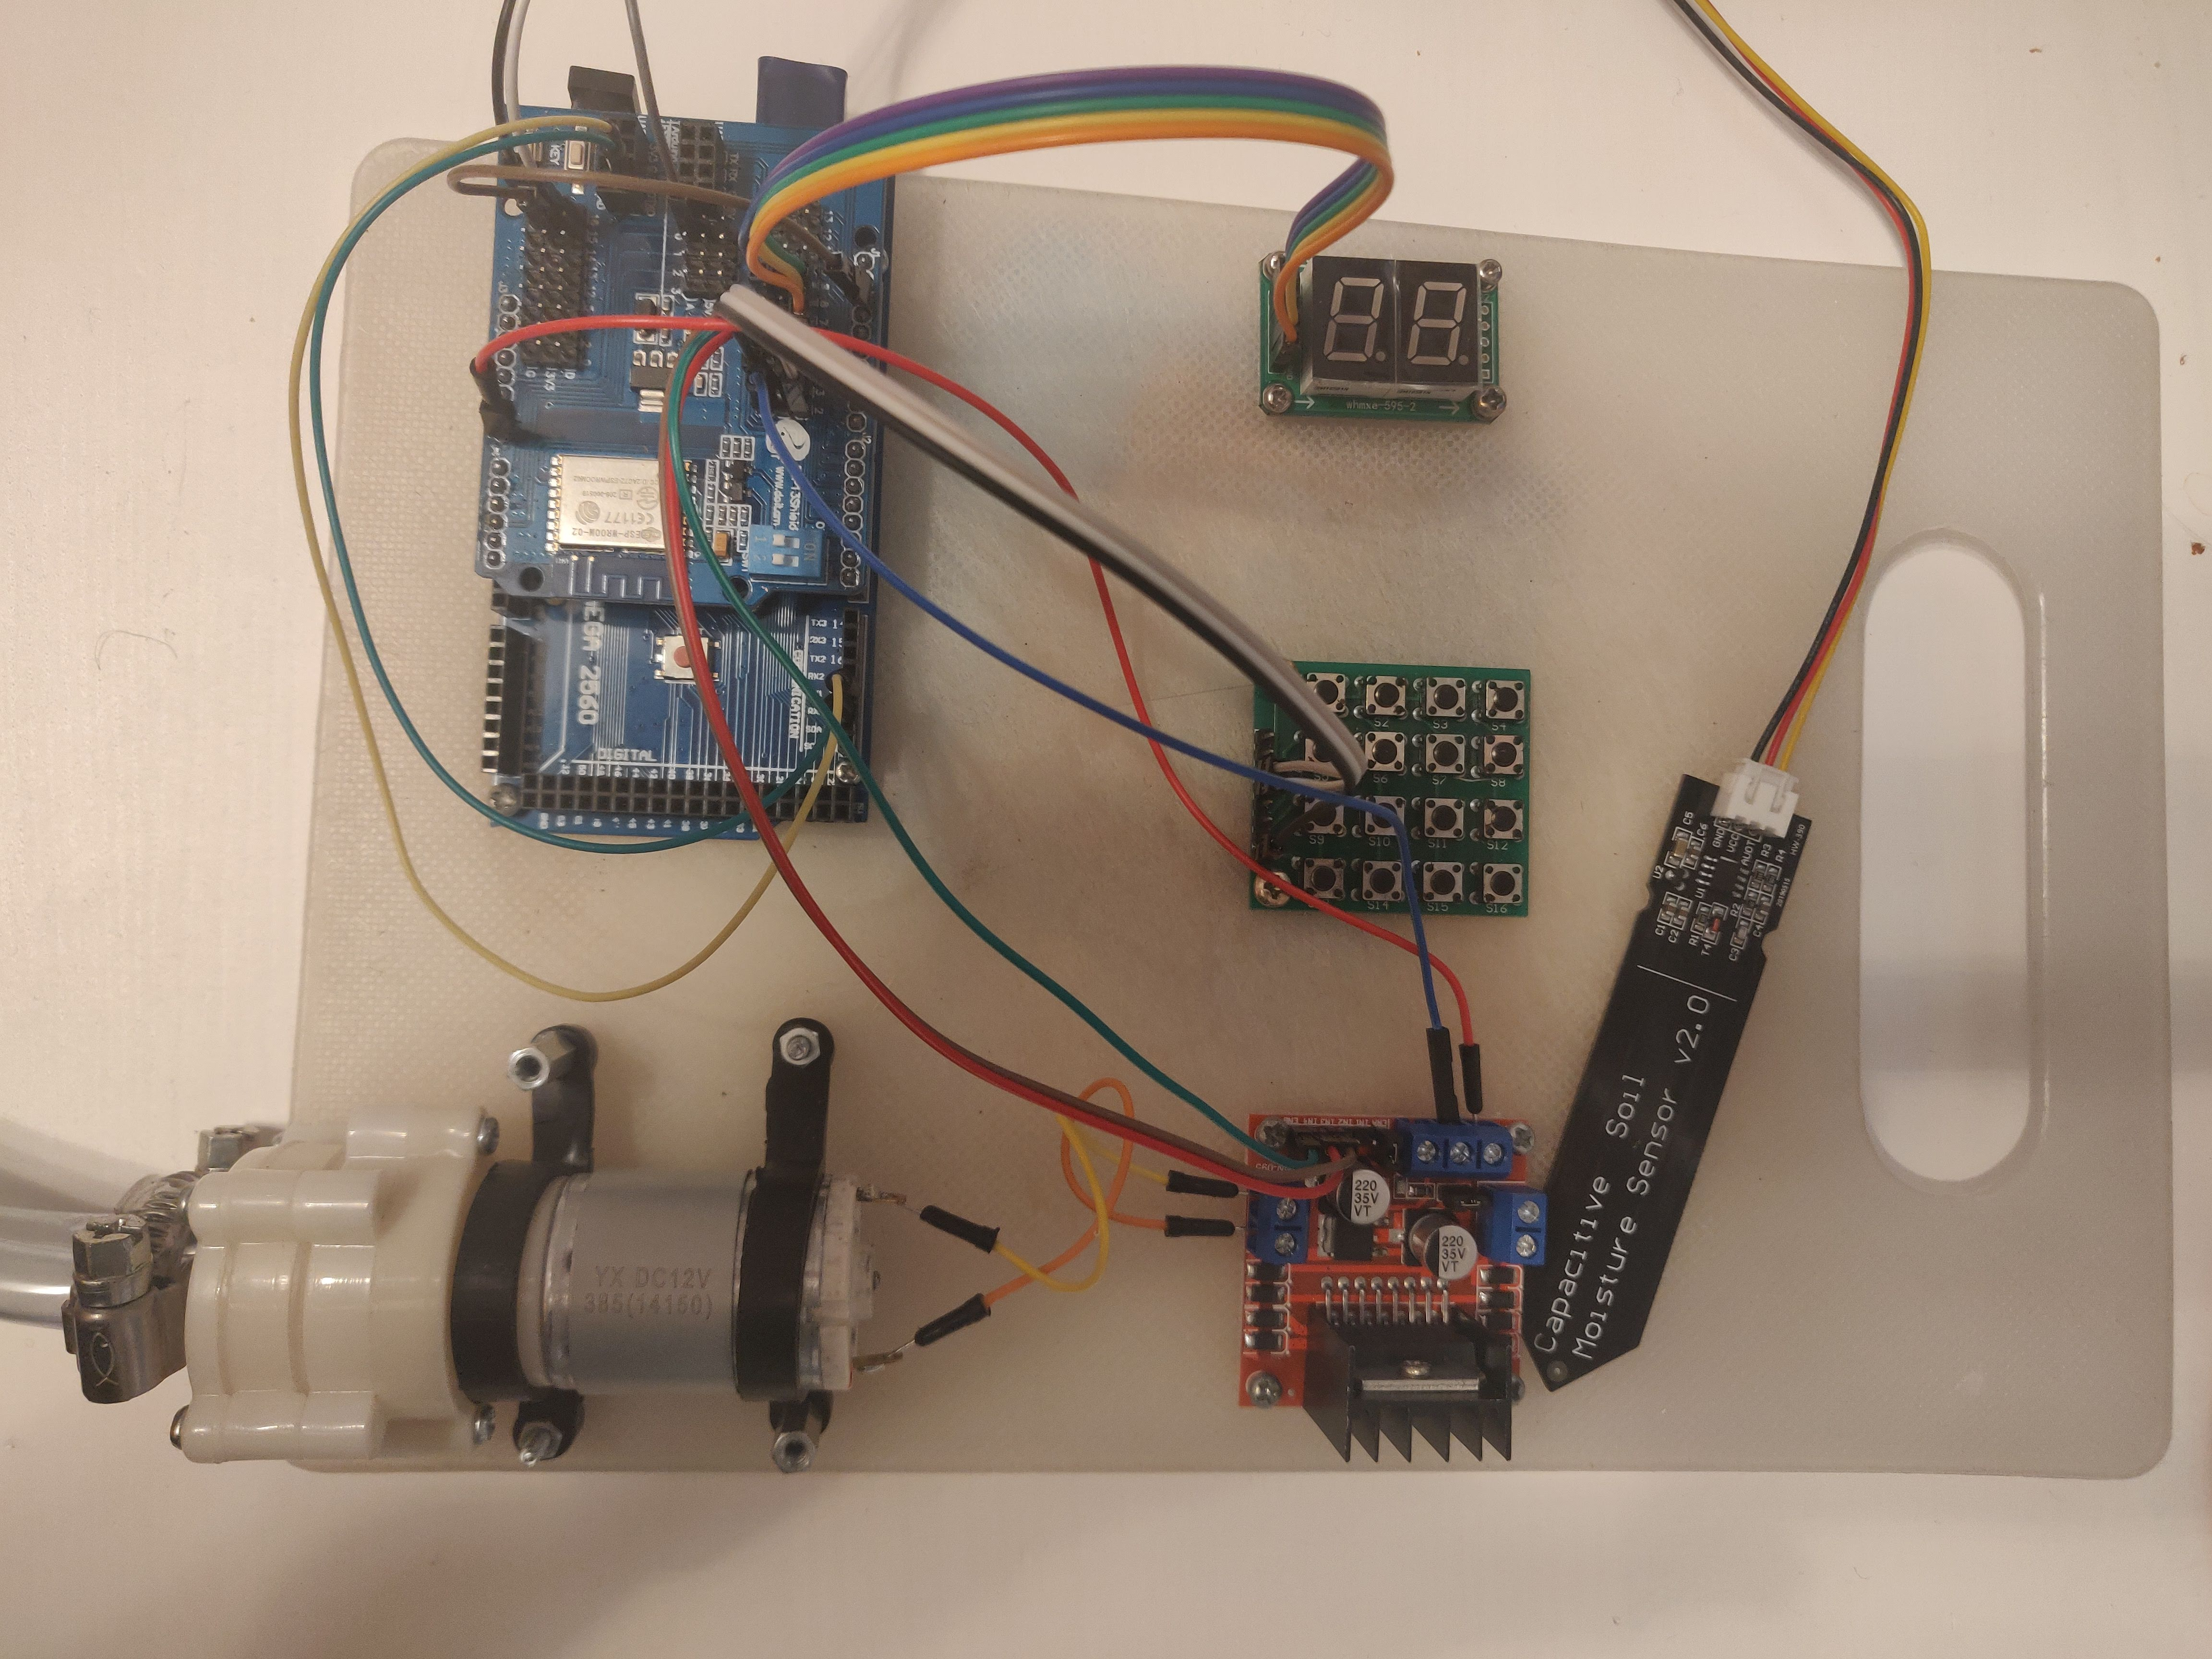
\includegraphics[width=\linewidth]{img/components.jpg}
    \caption{Picture of the components and their interconnection}
    \label{fig:components}
\end{figure}

Figure \ref{fig:hardware_diagram} shows the components used in the project. Figure \ref{fig:components} shows the real circuit.

An \textbf{Arduino Mega 2560} was used for controlling the moisture level. The program is uploaded on it. It receives 12V power through the DC jack.

For wireless communication a \textbf{DoIt ESP-13 Wi-Fi shield} was used. The AT firmware was uploaded to its ESP8266 chip. On figure \ref{fig:hardware_diagram} a different ESP component appears, because of the limitation in the design program. The voltage level shifters and regulators were hidden from the diagram because it is part of the shield. Therefore the TX and RX is directly connected to RX and TX of Arduino and the 5V port is unconnected on the image.

A 12V \textbf{water pump} was used for supplying water to the plants. This component works like a DC motor. Therefore it is represented as a motor on the image.

The pump needs a motor driver. Thus the \textbf{L298n motor driver} was added to the circuit. Its 12V power source is the external input voltage of the Arduino (VIN). The direction of the motor is hardwired, to pump only in one direction. The enable pin however is connected to the D6 pin of the Arduino board. Through this the microcontroller can turn on/off the pump or set its speed by using PWM.

A \textbf{capacitive moisture level sensor} was connected to the A0 pin of the board. It's supply voltage is 3.3V. The component differs from the one on the image because its capacitive, it is a single rod, and it can be directly connected to the board.

Two \textbf{buttons} are connected to the interrupt pins of the board. They are used for setting the extreme sensor values. When they are pressed, the program reads the sensor value and updates the current parameter with it.


Two \textbf{seven segment displays} are connected to the circuit. Their anodes are connected to '1' so the program must specify only their cathodes. The module containing the display manages this by using two 74HC595 shift registers. Therefore the only wires that are connected to the board are the: SDI, SCLK, LOAD. Thus the internal implementation of the module is not present on the diagram.

\section{Software}

The main program is defined in \verb|controller.ino|. In the \verb|setup()| function it displays the ``SE'' characters on the seven segment display, and calls the setup functions of each module. It has a \textbf{suspend flag}. When it is set, the loop function immediately returns, thus the program not executing anything anymore.

To achieve parallelism, the ``Timer.h'' library was used, which calls the given methods after the specified duration, by using the \verb|millis()| function. This library was used for handling the timings of the moisture controller presented in section \ref{sec:control_fsm}. Its implementation can be found in the \verb|processing.ino| file.

The \verb|config.h| file contains the constants of the program and also the application parameters. The \verb|Settings| data structure contains those parameters that can be modified by the user. The settings are read from the EEPROM and updated every time the field values change. The \verb|settings.ino| file implements the saving, loading and printing of this structure.

The \verb|moisture_sensor.ino| file handles the operations on the capacitive  soil moisture level sensor. It provides functions for reading the sensor value, handles the conversion  between the sensor value, the voltage value and the percentage. It also provides two functions for updating the two extreme sensor values.

The \verb|interrupts.ino| file configures the two buttons to trigger the interrupts. It also implements the interrupt service routines of them. These functions need to apply debouncing first, then they call the previously mentioned functions for updating the extreme values.

The \verb|pump.ino| file contains the functions for handling hte pump operations.

The \verb|display.ino| file handles the printing of characters and numbers to the seven segment displays. It contains a lookup table for all printable characters.

The \verb|error.h| contains an enum with all the system errors and their string representations. These are the errors that can be shown on the seven segment displays. The `\verb|error.ino| file contains the function which displays an error on the display, then it sets the \textit{suspend flag}.

The ``WiFiEsp.h'' library was used for the serial communication with the ESP8266 module, using the AT commands. In \verb|wifi.ino| functions are implemented which handle the setup of the module, the printing of the Wi-Fi data and the receiving of the clients. The latter function is called in the \verb|loop()| method of the main program. When the ESP module opens a socket this function receives a client object and reads the HTTP request character-by-character. The finite-state-machine described in \ref{sec:http_fsm} was used for parsing the input and saving the HTTP request type and the endpoint.

The requests are handled by the functions of the \verb|endpoints.ino| file. The \verb|handleRequest()| function receives a client, the request type and the endpoint, and routes it to the other methods. These function each implement and endpoint individually. The list of the endpoints and the corresponding functions can be seen in table \ref{tab:enpoints}. To send an receive JSON messages, the ``ArduinoJson.h'' library was used.

In case of an unparsable input, an inexisting endpoint, an unavailable request type or invalid input the corresponding HTTP responses are returned: BAD REQUEST, NOT FOUND, METHOD NOT ALLOWED, UNPROCESSABLE ENTITY. If the functions are executed correctly, the OK response is returned.

The \verb|http.h| header contains the HTTP status codes which are used in the program with their string representation. The \verb|http.ino| file implements methods for sending HTTP responses

The \verb|util.h| file contains the utility functions, such as \verb|average()|, which calculates the average of returned values when calling a function repeated times. This is used for reading the sensor data.

\subsubsection{Debugging}

For debugging, the program prints values to its main serial port, which is connected to the USB port. When the program starts, it prints the saved configuration values and also other data related to the wifi connection, such as its local ip address.


\begin{table}[ht]
 \centering
 \begin{tabular}{| l | c | l | p{0.55\linewidth} |} 
    \hline
    Function & Request & Endpoint & Action \\ [0.5ex] 
    \hline\hline
    getRoot & GET & / & Show all endpoints\\ 
    \hline
    getSensor & GET & /sensor & Show the parameters related to the sensor readings:
    \begin{itemize}
     \item The range of valid values: min and max
     \item The extreme values: dry and wet
     \item The threshold percentage
    \end{itemize}\\ 
    \hline
    updateSensor & PATCH & /sensor & Update the parameters. Each specified input value is validated. The HTTP response tells if the execution was a success\\ 
    \hline
    getSensor & GET & /moisture & Show the current moisture value in multiple formats:
    \begin{itemize}
     \item Raw sensor reading
     \item Voltage 
     \item Percentage
    \end{itemize}\\ 
    \hline
    getTiming & GET & /timing & Show the parameters related to the timing:
    \begin{itemize}
     \item sensorReactionTime - parameter of the controller
     \item pumpingTime - parameter of the controller
     \item delayBetweenChecks - parameter of the controller
     \item displayRefreshPeriod - specifies the waiting period after updating the percentage on the 7-segment display
    \end{itemize}\\ 
    \hline
    updateTiming & PATCH & /timing & Update the parameters. Each specified input value is validated. The HTTP response tells if the execution was a success\\ [1ex] 
    \hline
 \end{tabular}
 \caption{The endpoints of the web server and the corresponding functions which implement them}
 \label{tab:enpoints}
\end{table}








\chapter{Testing and validation}

Before the development I tested each component to learn about how they work and how can I use them in the project. This reasearch process required a significant amount of time, especially for the ESP8266 Wi-Fi modules, for which I had to understand the flashing process. Below are enumerated the design decisions I took and the questions I had.

Although having a spare NodeMCU, an Arduino Mega was chosen for the microcontroller. The initial plan was to support multiple plants, which required multiple analog pins, but only one was accessible by the NodeMCU. However by using a multiplexer for the analog input or using an operational amplifier for controlling the pump, this limitation would have been resolved thus I could have embraced all the benefits of writing directly the code to the ESP8266.

By not choosing the NodeMCU additional questions were raised. I needed to decide whether to use the ESP-01 Wi-Fi module which required voltage level shifters and therefore additional soldering, or to use the DoIt ESP-13 Wi-Fi shield which handles all of these problems, but in exchange, it does not provide acces to the VIN and AREF ports. I chose the solution which can be executed the fastest. I soldered to sockets to the Wi-Fi shield. This way I can connect this two pins with regular jumper wires.

Another decision was that I used the AT firmware on the ESP module. At first I thought about writing my own firmware. Then I realized that it requires too much time, because this way I must implement my own data sending protocol through the serial port. So I chose the AT commands. But it was not simple to use them. Fortunately, the ``WiFiEsp'' library provides a higher level API for a few operations with the module. The only thing left for me was to parse the HTTP request byte-by-byte to get the request type and the endpoint. Then I could implement regularly the endpoints, like if I used the NodeMCU.

Another significant change in plan was the choice of the water pump. Initially the pump I used worked on 5 volts, and it also changed polarity while rotating. However all the tutorials on the internet connected the pump to a simple relay instead of a H-bridge. Therefore I calmly connected the pump to the arduino (without using a relay), which was fried a few seconds later. After that I used the L298n motor driver. But because of the operating voltage of the pump was 5V, the motor driver overheated. At this moment I bought a new pump which works on 12V.

Most of the decisions was taken before or during the development. After each module was implemented I tested for correct behavior. The first functional state of the system corresponds to the final state.

\section{Endpoint testing}

The endpoints were tested by using the Postman program. Through this, one can send HTTP requests of all types, with or without body, and see the responses. This way was verified the behavior and the proper reaction of the system.

\chapter{Conclusion}




\section{Ideas for a new design}

Through the experiences gained during the development I obtained more insights on what design decisions would have been better for solving the same problem.

For a new design I would consider:

\begin{itemize}
 \item Operational amplifiers for controlling the moisture levels
 \item NodeMCU for the Wireless communication, application logic and for supplying the reference voltages for the operational amplifiers
 \item Master-slave communication which allows to control more plants than the number of pins on the microcontroller without the need of using multiplexers.
\end{itemize}


\section{Ideas for improvements}

The following improvements would benefit both the new and the current design:

\begin{itemize}
 \item Using the calibration method presented in \cite{Hrisko20} to compute the volumetric water content
 \item Using an SD card to store the configuration data and the sensor readings. Thus having a history of moisture levels which could be queried through a new endpoint.
 \item Using a water level sensor to stop pumping when the water tank is empty, and instead alert the user.
 \item Creating a client interface: mobile or web.
\end{itemize}


\section{Conclusions}

This project was a great opportunity to apply in practice the concepts I learned at the university \cite{Danescu2018} and to discover more components and techniques.

I did not take the best design decision when I did not choose the NodeMCU and the operational amplifier. But that only provided disadvantage during the initial development. Now the program can be easily extended by implementing the function of a new endpoint and calling it in the routing method.

The purpose was fulfilled. The end result is a fully-functioning automatized irrigation station which can be configured using a RESTful API. It solves the real life problem of irrigating a plant according to its needs. This solution can help anybody who needs this kind of automation in his/her plant's life.


\Urlmuskip=0mu plus 1mu
%\addcontentsline {toc}{chapter}{Bibliography} 
\bibliographystyle{IEEEtran} 
\bibliography{documentation}%same file name as for .bib

\end{document}
